\documentclass{article}
\usepackage{geometry}
\geometry{
	a4paper,
	left=2.5cm,   
	right=2.5cm,   
	top=2.5cm,      
	bottom=2.5cm,  
	headheight=13.6pt
}

% 最简单、最稳定的中文方案（自动适配系统，永不报错）
\usepackage[UTF8, scheme=plain]{ctex}

% 设置英文默认字体为 Times New Roman
\usepackage{fontspec}
\setmainfont{Times New Roman}

\usepackage{amsmath}
\usepackage{amssymb}
\usepackage{booktabs}
\usepackage{caption}
\usepackage{setspace}
\onehalfspacing
\setlength{\parskip}{4pt}

\usepackage{array}
\usepackage{listings}
\usepackage{graphicx}
\usepackage{enumitem}
\usepackage{subcaption}
\usepackage{multirow}
\usepackage{mathrsfs}
\usepackage{bm}
\usepackage{xcolor}
\usepackage{colortbl}

\usepackage{tikz}
\usepackage{tikz-3dplot}
\usetikzlibrary{
	arrows.meta, 
	calc, 
	patterns, 
	decorations.pathmorphing, 
	backgrounds, 
	positioning, 
	fit, 
	shapes.geometric, 
	intersections, 
	through, 
	angles, 
	quotes,
	plotmarks
}

%目录超链接
\usepackage{hyperref}
\hypersetup{
	colorlinks=true,
	linkcolor=black,
	filecolor=magenta,      
	urlcolor=cyan,
}
\usepackage{tocloft}
\setlength{\cftbeforesecskip}{2ex}
\setlength{\cftbeforesubsecskip}{1ex}
\setlength{\cftbeforesubsubsecskip}{1ex}

% 定义代码颜色
\definecolor{codegreen}{rgb}{0,0.6,0}
\definecolor{NavyBlue}{RGB}{0,0,128}
\definecolor{PineGreen}{RGB}{1,121,111}

% 配置 listings 环境
\lstset{
	language=TeX,
	tabsize=4,
	captionpos=b,
	numbers=left,
	numbersep=1em,
	sensitive=true,
	showtabs=false,
	frame=shadowbox,
	breaklines=true,
	keepspaces=true,
	showspaces=false,
	showstringspaces=false,
	breakatwhitespace=false,
	basicstyle=\ttfamily\normalsize,
	keywordstyle=\color{NavyBlue},
	commentstyle=\color{codegreen},
	numberstyle=\color{black},
	stringstyle=\color{PineGreen!90!black},
	rulesepcolor=\color{red!20!green!20!blue!20},
	escapeinside={/@}{@/},
}

\definecolor{LightGreen}{rgb}{0.9, 0.95, 0.9}
\definecolor{LightBlue}{RGB}{229, 238, 255}
\definecolor{LightPink}{RGB}{255, 229, 237}

\captionsetup[table]{
	justification=centering,
	labelsep=quad,
	font={bf}
}
\captionsetup[figure]{
	justification=centering,
	labelsep=quad,
	font={bf}
}
\captionsetup[subfigure]{
	font={bf}
}

\begin{document}

\begin{center}
	{\LARGE \textbf{LaTeX 零基础画图教程}} \\[0.5cm]
	{\large {\kaishu 石继楷 \quad 编写}} \\[0.3cm]
	{\normalsize 2026年7月26日}
\end{center}

\tableofcontents
\newpage

\section{引言}
本教程使用 \texttt{TikZ} 与 \texttt{tikz-3dplot} 宏包，从零开始讲解如何在 LaTeX 中绘制数学图形。内容包括：
\begin{itemize}
	\item 平面图形：直线、坐标系、三角形、圆、椭圆、抛物线、双曲线以及各种标注技巧。
	\item 三维图形：三维坐标系、空间点、直线、平面、多面体、旋转体（线框示意）等。
\end{itemize}
因 \texttt{pgfplots}较难，全文不涉及\texttt{pgfplots}。

\section{准备工作}
在导言区需加载以下宏包：
\begin{lstlisting}
\usepackage{tikz}
\usepackage{tikz-3dplot}
\usetikzlibrary{
	arrows.meta, calc, patterns, intersections, 
	through, angles, quotes, decorations.pathmorphing
}
\end{lstlisting}

\section{平面绘图基础}

使用 \verb|\draw| 绘制直线。标记点有两种方式：

\begin{itemize}
	\item \textbf{直接标记}：\verb|\fill (0,0) circle (2pt);| 画一个点，但该点没有名称，后续无法引用。
	\item \textbf{命名后批量标记}：先用 \verb|\coordinate| 定义点，再用 \verb|\foreach| 统一画点。
\end{itemize}

\textbf{推荐做法}：对于会被多次引用的点，务必命名；对于只用一次的点，可直接用 \verb|\fill|。

\begin{lstlisting}
\begin{tikzpicture}
	% 命名点
	\coordinate (A) at (0,0);
	\coordinate (B) at (4,0);
	\coordinate (C) at (1,3);
	
	% 画三角形
	\draw (A) -- (B) -- (C) -- cycle;
	
	% 批量标记所有点
	\foreach \p/\pos in {A/below left,B/below right,C/above}
	\fill (\p) circle (2pt) node[\pos] {$\p$};
	
	% 也可以单独画一个无名点
	\fill (1.5,1) circle (2pt) node[below] {无名点$D$};
\end{tikzpicture}
\end{lstlisting}
\begin{center}
\begin{tikzpicture}
	% 命名点
	\coordinate (A) at (0,0);
	\coordinate (B) at (4,0);
	\coordinate (C) at (1,3);
	
	% 画三角形
	\draw (A) -- (B) -- (C) -- cycle;
	
	% 批量标记所有点
	\foreach \p/\pos in {A/below left,B/below right,C/above}
	\fill (\p) circle (2pt) node[\pos] {$\p$};
	
	% 也可以单独画一个无名点
	\fill (1.5,1) circle (2pt) node[below] {无名点$D$};
\end{tikzpicture}
\end{center}


\subsection{直线与点}
\begin{lstlisting}
\begin{tikzpicture}
	\draw[->] (-1,0) -- (4,0) node[right] {$x$};
	\draw[->] (0,-1) -- (0,3) node[above] {$y$};
	\draw[thick, blue] (0.5,0.5) -- (3,2.5);
	\fill[red] (0.5,0.5) circle (2pt) node[below left] {$A$};
	\fill[red] (3,2.5) circle (2pt) node[above right] {$B$};
\end{tikzpicture}
\end{lstlisting}

\begin{center}
	\begin{tikzpicture}[scale=1]
		\draw[->] (-1,0) -- (4,0) node[right] {$x$};
		\draw[->] (0,-1) -- (0,3) node[above] {$y$};
		\draw[thick, blue] (0.5,0.5) -- (3,2.5);
		\fill[red] (0.5,0.5) circle (2pt) node[below left] {$A$};
		\fill[red] (3,2.5) circle (2pt) node[above right] {$B$};
	\end{tikzpicture}
\end{center}

\subsection{坐标系与网格}
使用 TikZ 的 \verb|\draw| 和 \verb|grid| 绘制带网格的坐标系。

\begin{lstlisting}
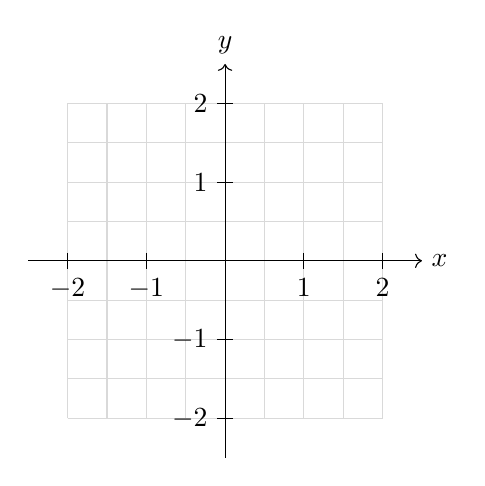
\begin{tikzpicture}
	% 网格
	\draw[step=0.5, gray!30, thin] (-2,-2) grid (2,2);
	% 坐标轴
	\draw[->] (-2.5,0) -- (2.5,0) node[right] {$x$};
	\draw[->] (0,-2.5) -- (0,2.5) node[above] {$y$};
	% 刻度标签（示例）
	\foreach \x in {-2,-1,1,2}
	\draw (\x,0.1) -- (\x,-0.1) node[below] {$\x$};
	\foreach \y in {-2,-1,1,2}
	\draw (0.1,\y) -- (-0.1,\y) node[left] {$\y$};
\end{tikzpicture}
\end{lstlisting}

\begin{center}
	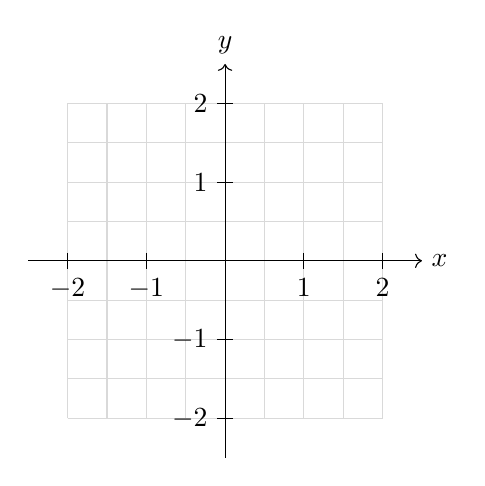
\begin{tikzpicture}
		\draw[step=0.5, gray!30, thin] (-2,-2) grid (2,2);
		\draw[->] (-2.5,0) -- (2.5,0) node[right] {$x$};
		\draw[->] (0,-2.5) -- (0,2.5) node[above] {$y$};
		\foreach \x in {-2,-1,1,2}
		\draw (\x,0.1) -- (\x,-0.1) node[below] {$\x$};
		\foreach \y in {-2,-1,1,2}
		\draw (0.1,\y) -- (-0.1,\y) node[left] {$\y$};
	\end{tikzpicture}
\end{center}

\subsection{三角形与辅助线}
使用 \verb|\draw| 的闭合路径绘制多边形，可填充颜色，并可计算中点、垂线等。

\begin{lstlisting}
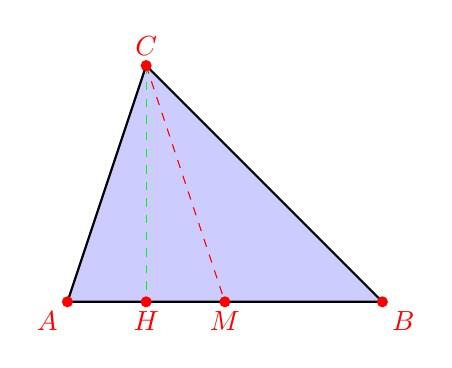
\begin{tikzpicture}
	\coordinate (A) at (0,0);
	\coordinate (B) at (4,0);
	\coordinate (C) at (1,3);
	\fill[blue!20] (A) -- (B) -- (C) -- cycle;
	\draw[thick] (A) -- (B) -- (C) -- cycle;
	\coordinate (M) at ($(A)!0.5!(B)$);
	\draw[dashed, red] (C) -- (M);
	\coordinate (H) at ($(A)!(C)!(B)$);
	\draw[dashed, green] (C) -- (H);
	\foreach \p/\pos in {A/below left, B/below right, C/above, M/below, H/below}
	\fill[red] (\p) circle (2pt) node[\pos] {$\p$};
\end{tikzpicture}
\end{lstlisting}

\begin{center}
	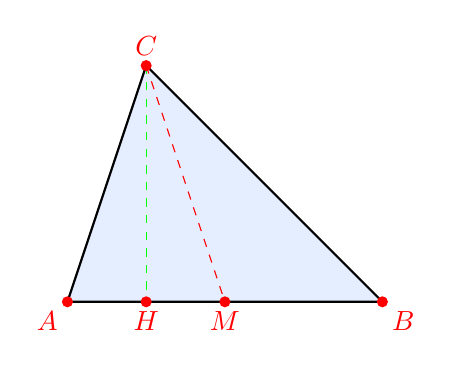
\begin{tikzpicture}
		\coordinate (A) at (0,0);
		\coordinate (B) at (4,0);
		\coordinate (C) at (1,3);
		\fill[LightBlue] (A) -- (B) -- (C) -- cycle;
		\draw[thick] (A) -- (B) -- (C) -- cycle;
		\coordinate (M) at ($(A)!0.5!(B)$);
		\draw[dashed, red] (C) -- (M);
		\coordinate (H) at ($(A)!(C)!(B)$);
		\draw[dashed, green] (C) -- (H);
		\foreach \p/\pos in {A/below left, B/below right, C/above, M/below, H/below}
		\fill[red] (\p) circle (2pt) node[\pos] {$\p$};
	\end{tikzpicture}
\end{center}

\newpage
\subsection{角度标注}
使用 \texttt{angles} 和 \texttt{quotes} 库方便标注角度。

\begin{lstlisting}
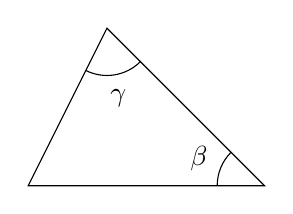
\begin{tikzpicture}
	\coordinate (A) at (0,0);
	\coordinate (B) at (3,0);
	\coordinate (C) at (1,2);
	\draw (A) -- (B) -- (C) -- cycle;
	\draw pic["$\beta$", draw, angle eccentricity=1.5, angle radius=0.6cm] 
	{angle = C--B--A};
	\draw pic["$\gamma$", draw, angle eccentricity=1.5, angle radius=0.6cm] 
	{angle = A--C--B};
\end{tikzpicture}
\end{lstlisting}

\begin{center}
	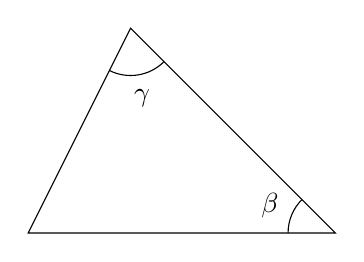
\begin{tikzpicture}[scale=1.3]
		\coordinate (A) at (0,0);
		\coordinate (B) at (3,0);
		\coordinate (C) at (1,2);
		\draw (A) -- (B) -- (C) -- cycle;
		\draw pic["$\beta$", draw, angle eccentricity=1.5, angle radius=0.6cm] 
		{angle = C--B--A};
		\draw pic["$\gamma$", draw, angle eccentricity=1.5, angle radius=0.6cm] 
		{angle = A--C--B};
	\end{tikzpicture}
\end{center}

\subsection{坐标系进阶：交点}
利用 \texttt{intersections} 库求两条曲线的交点。\textbf{注意：}必须确保两条路径确实相交，且路径名定义正确。本例使用直线 $y=x-1$ 与抛物线 $y=0.5x^2-1$，交于 $(0,-1)$ 和 $(2,1)$。

\begin{lstlisting}
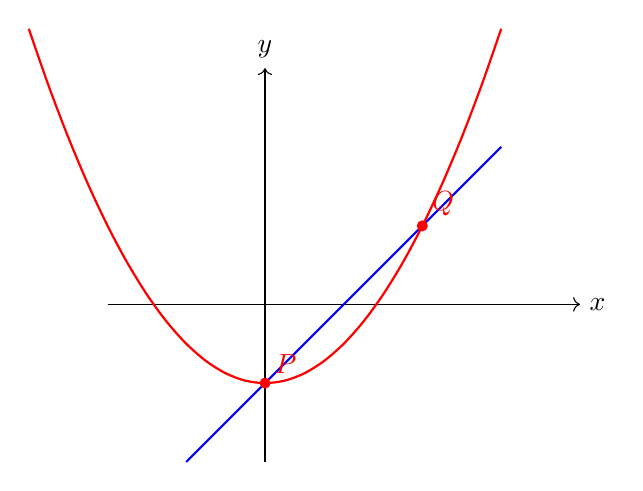
\begin{tikzpicture}
	\draw[->] (-2,0) -- (4,0) node[right]{$x$};
	\draw[->] (0,-2) -- (0,3) node[above]{$y$};
	\draw[name path=line, thick, blue] (-1,-2) -- (3,2);
	\draw[name path=parabola, thick, red, domain=-3:3, smooth, variable=\x] 
	plot ({\x}, {0.5*\x*\x - 1});
	\path [name intersections={of=line and parabola, by={P,Q}}];
	\fill[red] (P) circle (2pt) node[above right] {$P$};
	\fill[red] (Q) circle (2pt) node[above right] {$Q$};
\end{tikzpicture}
\end{lstlisting}

\begin{center}
	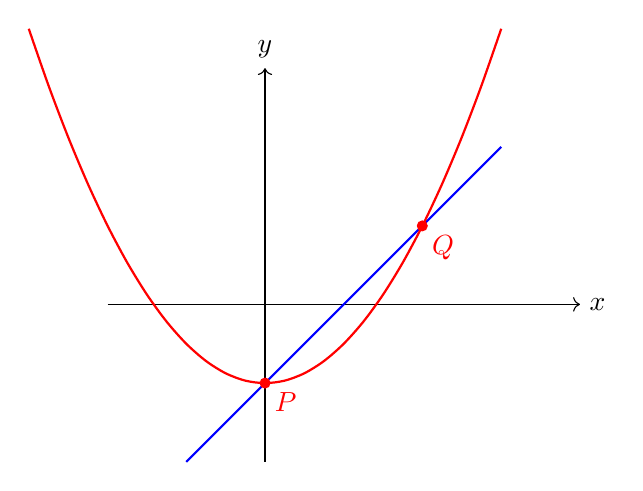
\begin{tikzpicture}[scale=1]
		\draw[->] (-2,0) -- (4,0) node[right]{$x$};
		\draw[->] (0,-2) -- (0,3) node[above]{$y$};
		\draw[name path=line, thick, blue] (-1,-2) -- (3,2);
		\draw[name path=parabola, thick, red, domain=-3:3, smooth, variable=\x] 
		plot ({\x}, {0.5*\x*\x - 1});
		\path [name intersections={of=line and parabola, by={P,Q}}];
		\fill[red] (P) circle (2pt) node[below right] {$P$};
		\fill[red] (Q) circle (2pt) node[below right] {$Q$};
	\end{tikzpicture}
\end{center}

或者手动定交点：

\begin{lstlisting}
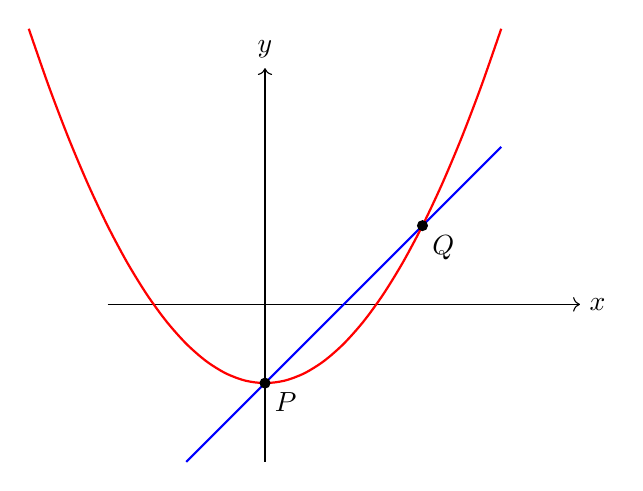
\begin{tikzpicture}
	\draw[->] (-2,0) -- (4,0) node[right]{$x$};
	\draw[->] (0,-2) -- (0,3) node[above]{$y$};
	
	% 画直线和抛物线
	\draw[thick, blue] (-1,-2) -- (3,2);
	\draw[thick, red, domain=-3:3, smooth, variable=\x] 
	plot ({\x}, {0.5*\x*\x - 1});
	
	% 手动标记交点（已知为 (0,-1) 和 (2,1)）
	\fill (0,-1) circle (2pt) node[below right] {$P$};
	\fill (2,1)  circle (2pt) node[below right] {$Q$};
\end{tikzpicture}
\end{lstlisting}

\begin{center}
	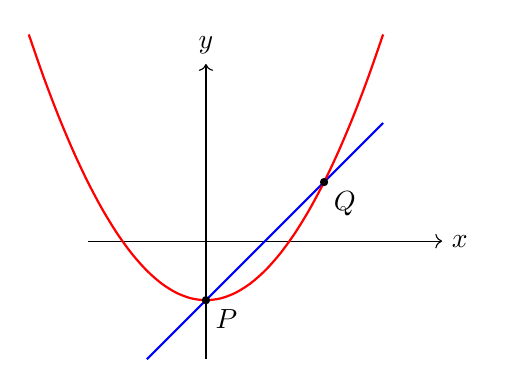
\begin{tikzpicture}[scale=0.75]
		\draw[->] (-2,0) -- (4,0) node[right]{$x$};
		\draw[->] (0,-2) -- (0,3) node[above]{$y$};
		
		% 画直线和抛物线
		\draw[thick, blue] (-1,-2) -- (3,2);
		\draw[thick, red, domain=-3:3, smooth, variable=\x] 
		plot ({\x}, {0.5*\x*\x - 1});
		
		% 手动标记交点（已知为 (0,-1) 和 (2,1)）
		\fill (0,-1) circle (2pt) node[below right] {$P$};
		\fill (2,1)  circle (2pt) node[below right] {$Q$};
	\end{tikzpicture}
\end{center}

\subsection{圆锥曲线}
\subsubsection{圆}
\vspace*{-10pt}
用 \verb|circle| 命令绘制圆。

\begin{lstlisting}
\begin{tikzpicture}
	\draw[->] (-3,0) -- (3,0) node[right] {$x$};
	\draw[->] (0,-3) -- (0,3) node[above] {$y$};
	\draw[thick, red] (0,0) circle (2);
	\fill (0,0) circle (1pt) node[below left] {$O$};
\end{tikzpicture}
\end{lstlisting}

\begin{center}
	\begin{tikzpicture}[scale=0.8]
		\draw[->] (-3,0) -- (3,0) node[right] {$x$};
		\draw[->] (0,-3) -- (0,3) node[above] {$y$};
		\draw[thick, red] (0,0) circle (2);
		\fill (0,0) circle (1pt) node[below left] {$O$};
	\end{tikzpicture}
\end{center}

\subsubsection{椭圆}
使用 TikZ 的 \verb|ellipse| 命令，简单直接。

\begin{lstlisting}
\begin{tikzpicture}
	\draw[->] (-3,0) -- (3,0) node[right] {$x$};
	\draw[->] (0,-2) -- (0,2) node[above] {$y$};
	\draw[thick, blue] (0,0) ellipse (2 and 1.2);
\end{tikzpicture}
\end{lstlisting}

\vspace*{-5pt}
\begin{center}
	\begin{tikzpicture}
		\draw[->] (-3,0) -- (3,0) node[right] {$x$};
		\draw[->] (0,-2) -- (0,2) node[above] {$y$};
		\draw[thick, blue] (0,0) ellipse (2 and 1.2);
	\end{tikzpicture}
\end{center}

\vspace*{-20pt}
\subsubsection{抛物线}
\vspace*{-5pt}
绘制 $y=x^2$ 等，也可绘制焦点和准线（使用 TikZ 的 'plot'）。

\begin{lstlisting}
\begin{tikzpicture}
	\draw[->] (-3,0) -- (3,0) node[right] {$x$};
	\draw[->] (0,-3) -- (0,3) node[above] {$y$};
	\draw[thick, orange, domain=-1.5:1.5, smooth, variable=\x] 
	plot ({\x*\x}, {2*\x});
	% /@ $x=t^2$ @/, /@ $y=2t \Rightarrow t=\dfrac{y}{2}$ @/ 代入1式.
	% /@ $\therefore x=(\dfrac{y}{2})^2 $@/
	% /@ $\therefore y^2=4x $@/
	\fill (-1,0) circle (2pt);
	\fill (1,0) circle(2pt) node[above]{$\text{焦点}(1,0)$};
	\draw[dashed] (-1,-3) -- (-1,3) node[left] {$x=-1$};
\end{tikzpicture}
\end{lstlisting}

\begin{center}
	\begin{tikzpicture}
		\draw[->] (-3,0) -- (3,0) node[right] {$x$};
		\draw[->] (0,-3) -- (0,3) node[above] {$y$};
		\draw[thick, orange, domain=-1.5:1.5, smooth, variable=\x] 
		plot ({\x*\x}, {2*\x});%y^2=4x
		\fill (-1,0) circle (2pt);
		\fill (1,0) circle(2pt) node[above]{$\text{焦点}(1,0)$};
		\draw[dashed] (-1,-3) -- (-1,3) node[left] {$x=-1$};
	\end{tikzpicture}
\end{center}

\subsubsection{双曲线}
使用 TikZ 的 \texttt{plot} 绘制两个分支，并添加渐近线。

\begin{lstlisting}
	\begin{tikzpicture}
		\draw[->, gray!40] (-4,0) -- (4,0) node[right] {$x$};
		\draw[->, gray!40] (0,-4) -- (0,4) node[above] {$y$};
		% 右支：x>=1，用y作自变量
		\draw[thick, DarkRed, domain=-3.5:3.5, smooth, variable=\y] plot ({sqrt(\y*\y+1)}, {\y});
		% 左支：x<=-1，用y作自变量
		\draw[thick, DarkRed, domain=-3.5:3.5, smooth, variable=\y] plot ({-sqrt(\y*\y+1)}, {\y});
		% 渐近线 y=x 和 y=-x
		\draw[dashed, gray!40] (-3.5,-3.5) -- (3.5,3.5);
		\draw[dashed, gray!40] (-3.5,3.5) -- (3.5,-3.5);
	\end{tikzpicture}
\end{lstlisting}

\begin{center}
	\begin{tikzpicture}[scale=0.9, baseline=(current bounding box.north)]
		\draw[->, gray!40] (-4,0) -- (4,0) node[right] {$x$};
		\draw[->, gray!40] (0,-4) -- (0,4) node[above] {$y$};
		% 右支：x>=1，用y作自变量
		\draw[thick, teal, domain=-3.5:3.5, smooth, samples=200, variable=\y] plot ({sqrt(\y*\y+1)}, {\y});
		% 左支：x<=-1，用y作自变量
		\draw[thick, teal, domain=-3.5:3.5, smooth, samples=200, variable=\y] plot ({-sqrt(\y*\y+1)}, {\y});
		% 渐近线 y=x 和 y=-x
		\draw[dashed, gray!40] (-3.5,-3.5) -- (3.5,3.5);
		\draw[dashed, gray!40] (-3.5,3.5) -- (3.5,-3.5);
	\end{tikzpicture}
\end{center}

\subsection{极坐标绘图（玫瑰线）}
使用 TikZ 的参数方程绘制极坐标曲线 $r=2\cos 3\theta$。

\begin{lstlisting}
\begin{tikzpicture}
	\draw[->] (-2.5,0) -- (2.5,0) node[right] {$x$};
	\draw[->] (0,-2.5) -- (0,2.5) node[above] {$y$};
	\draw[thick, red, domain=0:360, smooth, samples=200, variable=\t]
	plot ({2*cos(3*\t)*cos(\t)}, {2*cos(3*\t)*sin(\t)});
\end{tikzpicture}
\end{lstlisting}

\begin{center}
	\begin{tikzpicture}[scale=1.5]
		\draw[->] (-2.5,0) -- (2.5,0) node[right] {$x$};
		\draw[->] (0,-2.5) -- (0,2.5) node[above] {$y$};
		\draw[thick, red, domain=0:360, smooth, samples=200, variable=\t]
		plot ({2*cos(3*\t)*cos(\t)}, {2*cos(3*\t)*sin(\t)});
	\end{tikzpicture}
\end{center}

\subsection{三角函数图像}
使用 TikZ 的 `plot` 绘制正弦、余弦函数图像。

\begin{lstlisting}
	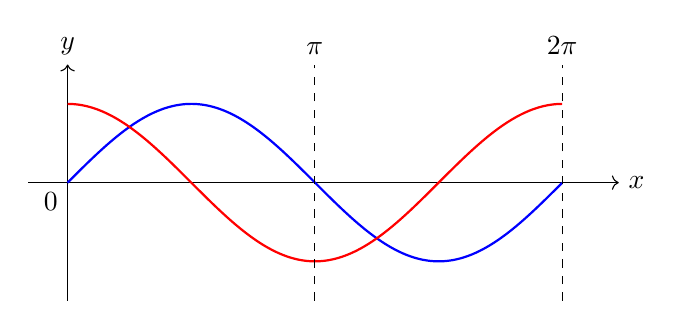
\begin{tikzpicture}
		\draw[->] (-0.5,0) -- (7,0) node[right] {$x$};
		\draw[->] (0,-1.5) -- (0,1.5) node[above] {$y$};
		\draw[thick, blue, domain=0:6.28, smooth, samples=100, variable=\x] 
		plot ({\x}, {sin(\x r)});  % 注意 r 表示弧度
		\draw[thick, red, domain=0:6.28, smooth, samples=100, variable=\x] 
		plot ({\x}, {cos(\x r)});
		\draw[dashed] (3.14,-1.5) -- (3.14,1.5) node[above] {$\pi$};
		\draw[dashed] (6.28,-1.5) -- (6.28,1.5) node[above] {$2\pi$};
		\draw (0,0) node[below left] {$0$};
	\end{tikzpicture}
\end{lstlisting}

\begin{center}
	\begin{tikzpicture}[scale=2]
		\draw[->] (-0.5,0) -- (7,0) node[right] {$x$};
		\draw[->] (0,-1.5) -- (0,1.5) node[above] {$y$};
		\draw[thick, blue, domain=0:6.28, smooth, samples=100, variable=\x] 
		plot ({\x}, {sin(\x r)});
		\draw[thick, red, domain=0:6.28, smooth, samples=100, variable=\x] 
		plot ({\x}, {cos(\x r)});
		\draw[dashed] (3.14,-1.5) -- (3.14,1.5) node[above] {$\pi$};
		\draw[dashed] (6.28,-1.5) -- (6.28,1.5) node[above] {$2\pi$};
		\draw (0,0) node[below left] {$0$};
	\end{tikzpicture}
\end{center}

\subsection{区域填充}
使用 \verb|\fill| 或 \verb|\clip| 填充曲线与坐标轴围成的区域。

\begin{lstlisting}
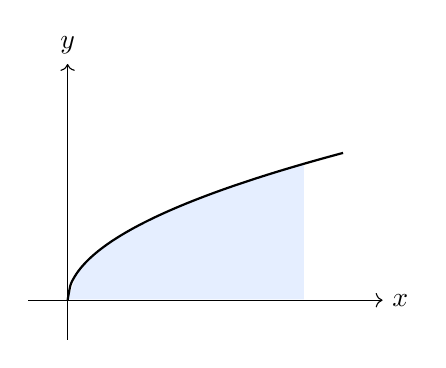
\begin{tikzpicture}
	\draw[->] (-0.5,0) -- (4,0) node[right] {$x$};
	\draw[->] (0,-0.5) -- (0,3) node[above] {$y$};
	\fill[LightBlue, domain=0:3, variable=\x] 
	(0,0.01) -- plot ({\x}, {sqrt(\x)}) -- (3,0.01) -- cycle;
	\draw[thick, domain=0:3.5, smooth, samples=100, variable=\x] 
	plot ({\x}, {sqrt(\x)});
\end{tikzpicture}
\end{lstlisting}

\begin{center}
	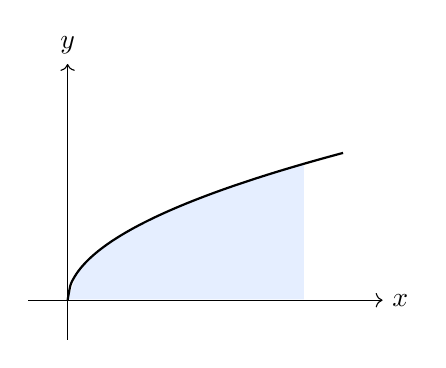
\begin{tikzpicture}
		\draw[->] (-0.5,0) -- (4,0) node[right] {$x$};
		\draw[->] (0,-0.5) -- (0,3) node[above] {$y$};
		\fill[LightBlue, domain=0:3, variable=\x] 
		(0,0.01) -- plot ({\x}, {sqrt(\x)}) -- (3,0.01) -- cycle;
		\draw[thick, domain=0:3.5, smooth, samples=100, variable=\x] 
		plot ({\x}, {sqrt(\x)});
	\end{tikzpicture}
\end{center}

\section{三维绘图}
\subsection{三维坐标系}
使用 \texttt{tikz-3dplot} 建立三维坐标系，方便绘制空间图形。

\begin{lstlisting}
\tdplotsetmaincoords{70}{120}
\begin{tikzpicture}[tdplot_main_coords, scale=2]
	\draw[->] (0,0,0) -- (2,0,0) node[below left]{$x$};
	\draw[->] (0,0,0) -- (0,2,0) node[right]{$y$};
	\draw[->] (0,0,0) -- (0,0,2) node[above]{$z$};
\end{tikzpicture}
\end{lstlisting}

\tdplotsetmaincoords{70}{120}
\begin{center}
	\begin{tikzpicture}[tdplot_main_coords, scale=1.8]
		\draw[->] (0,0,0) -- (2,0,0) node[below left]{$x$};
		\draw[->] (0,0,0) -- (0,2,0) node[right]{$y$};
		\draw[->] (0,0,0) -- (0,0,2) node[above]{$z$};
	\end{tikzpicture}
\end{center}

\newpage
\subsection{空间点与直线}
在三维坐标中绘制点、直线。

\begin{lstlisting}
\tdplotsetmaincoords{70}{120} %观察三位图形的角度
\begin{tikzpicture}[tdplot_main_coords]
	\draw[->] (0,0,0) -- (2,0,0) node[below left]{$x$};
	\draw[->] (0,0,0) -- (0,2,0) node[right]{$y$};
	\draw[->] (0,0,0) -- (0,0,2) node[above]{$z$};
	\coordinate (A) at (1,1,1);
	\coordinate (B) at (1.5,0.5,1.5);
	\draw[thick, blue] (A) -- (B);
	\fill[red] (A) circle (1.5pt) node[above] {$A$};
	\fill[red] (B) circle (1.5pt) node[above] {$B$};
\end{tikzpicture}
\end{lstlisting}

\tdplotsetmaincoords{70}{120}
\begin{center}
	\begin{tikzpicture}[tdplot_main_coords, scale=2]
		\draw[->] (0,0,0) -- (2,0,0) node[below left]{$x$};
		\draw[->] (0,0,0) -- (0,2,0) node[right]{$y$};
		\draw[->] (0,0,0) -- (0,0,2) node[above]{$z$};
		\coordinate (A) at (1,1,1);
		\coordinate (B) at (1.5,0.5,1.5);
		\draw[thick, blue] (A) -- (B);
		\fill[red] (A) circle (1.5pt) node[above] {$A$};
		\fill[red] (B) circle (1.5pt) node[above] {$B$};
	\end{tikzpicture}
\end{center}

\subsection{空间中的三角形与平面}
绘制三维三角形并填充半透明面，展示空间平面。

\begin{lstlisting}
\tdplotsetmaincoords{70}{120}
\begin{tikzpicture}[tdplot_main_coords, scale=2]
	\draw[->] (0,0,0) -- (2,0,0) node[below left]{$x$};
	\draw[->] (0,0,0) -- (0,2,0) node[right]{$y$};
	\draw[->] (0,0,0) -- (0,0,2) node[above]{$z$};
	\coordinate (A) at (0.5,0.5,0);
	\coordinate (B) at (1.5,0.5,0);
	\coordinate (C) at (1,1,1.2);
	\fill[blue!30, opacity=0.5] (A) -- (B) -- (C) -- cycle;
	\draw[thick] (A) -- (B) -- (C) -- cycle;
	\foreach \p/\pos in {A/below, B/below, C/above}
	\fill[red] (\p) circle (1.5pt) node[\pos] {$\p$};
\end{tikzpicture}
\end{lstlisting}

\tdplotsetmaincoords{70}{120}
\begin{center}
	\begin{tikzpicture}[tdplot_main_coords, scale=2]
		\draw[->] (0,0,0) -- (2,0,0) node[below left]{$x$};
		\draw[->] (0,0,0) -- (0,2,0) node[right]{$y$};
		\draw[->] (0,0,0) -- (0,0,2) node[above]{$z$};
		\coordinate (A) at (0.5,0.5,0);
		\coordinate (B) at (1.5,0.5,0);
		\coordinate (C) at (1,1,1.2);
		\fill[blue!30, opacity=0.5] (A) -- (B) -- (C) -- cycle;
		\draw[thick] (A) -- (B) -- (C) -- cycle;
		\foreach \p/\pos in {A/below, B/below, C/above}
		\fill[red] (\p) circle (1.5pt) node[\pos] {$\p$};
	\end{tikzpicture}
\end{center}

\subsection{三维多面体：正方体}
绘制一个带虚线的正方体，展示隐藏边。

\begin{lstlisting}
\tdplotsetmaincoords{70}{120}
\begin{tikzpicture}[tdplot_main_coords, scale=4]
	\coordinate (A) at (0,0,0);
	\coordinate (B) at (1,0,0);
	\coordinate (C) at (1,1,0);
	\coordinate (D) at (0,1,0);
	\coordinate (E) at (0,0,1);
	\coordinate (F) at (1,0,1);
	\coordinate (G) at (1,1,1);
	\coordinate (H) at (0,1,1);
	\draw[thick] (A) -- (B) -- (C) -- (D) -- cycle;
	\draw[thick] (E) -- (F) -- (G) -- (H) -- cycle;
	\draw[thick] (A) -- (E) (B) -- (F) (C) -- (G) (D) -- (H);
	\foreach \p/\pos in {A/above left,B/below left,C/below,D/right,E/above,F/left,G/above,H/above right}
	\fill (\p) circle (0.5pt) node[\pos] {$\p$};
\end{tikzpicture}
\end{lstlisting}

\tdplotsetmaincoords{70}{120}
\begin{center}
	\begin{tikzpicture}[tdplot_main_coords, scale=4]
		\coordinate (A) at (0,0,0);
		\coordinate (B) at (1,0,0);
		\coordinate (C) at (1,1,0);
		\coordinate (D) at (0,1,0);
		\coordinate (E) at (0,0,1);
		\coordinate (F) at (1,0,1);
		\coordinate (G) at (1,1,1);
		\coordinate (H) at (0,1,1);
		\draw[thick] (A) -- (B) -- (C) -- (D) -- cycle;
		\draw[thick] (E) -- (F) -- (G) -- (H) -- cycle;
		\draw[thick] (A) -- (E) (B) -- (F) (C) -- (G) (D) -- (H);
		\foreach \p/\pos in {A/above left,B/below left,C/below,D/right,E/above,F/left,G/above,H/above right}
		\fill (\p) circle (0.5pt) node[\pos] {$\p$};
	\end{tikzpicture}
\end{center}

\subsection{三维旋转体线框示意（圆锥、圆柱）}
使用纯 TikZ 绘制三维线框，展示常见旋转体的轮廓。

\vspace*{-10pt}
\paragraph{圆锥}
绘制底面圆和顶点，以及几条母线。
\begin{lstlisting}
\tdplotsetmaincoords{70}{120}
\begin{tikzpicture}[tdplot_main_coords, scale=1.5]
	\draw[->] (0,0,0) -- (2,0,0) node[below left]{$x$};
	\draw[->] (0,0,0) -- (0,2,0) node[right]{$y$};
	\draw[->] (0,0,0) -- (0,0,2) node[above]{$z$};
	% 底面圆
	\tdplotdrawarc{(0,0,0)}{1}{0}{360}{}{}
	%\tdplotdrawarc{中心点}{半径}{起始角度}{终止角度}{样式}{节点内容}
	% 顶点
	\coordinate (V) at (0,0,1.8);
	\fill (V) circle (1pt) node[right] {$V$};
	% 母线（画四条）
	\foreach \a in {0,90,180,270}
	\draw (V) -- ({cos(\a)}, {sin(\a)}, 0);
\end{tikzpicture}
\end{lstlisting}

\tdplotsetmaincoords{70}{120}
\begin{center}
	\begin{tikzpicture}[tdplot_main_coords, scale=1.5]
		\draw[->] (0,0,0) -- (2,0,0) node[below left]{$x$};
		\draw[->] (0,0,0) -- (0,2,0) node[right]{$y$};
		\draw[->] (0,0,0) -- (0,0,2.5) node[above]{$z$};
		\tdplotdrawarc{(0,0,0)}{1}{0}{360}{}{}
		\coordinate (V) at (0,0,1.8);
		\fill (V) circle (1pt) node[right] {$V$};
		\foreach \a in {0,90,180,270}
		\draw (V) -- ({cos(\a)}, {sin(\a)}, 0);
	\end{tikzpicture}
\end{center}

\paragraph{圆柱}
绘制上下底面圆和竖直线。
\begin{lstlisting}
\tdplotsetmaincoords{70}{120}
\begin{tikzpicture}[tdplot_main_coords, scale=1.5]
	\draw[->] (0,0,0) -- (2,0,0) node[below left]{$x$};
	\draw[->] (0,0,0) -- (0,2,0) node[right]{$y$};
	\draw[->] (0,0,0) -- (0,0,2) node[above]{$z$};
	% 下底面
	\tdplotdrawarc{(0,0,0)}{1}{0}{360}{}{}
	% 上底面
	\tdplotdrawarc{(0,0,1.5)}{1}{0}{360}{}{}
	% 母线（四条竖线）
	\foreach \a in {0,90,180,270}
	\draw ({cos(\a)}, {sin(\a)}, 0) -- ({cos(\a)}, {sin(\a)}, 1.5);
\end{tikzpicture}
\end{lstlisting}

\tdplotsetmaincoords{70}{120}
\begin{center}
	\begin{tikzpicture}[tdplot_main_coords, scale=1.5]
		\draw[->] (0,0,0) -- (2,0,0) node[below left]{$x$};
		\draw[->] (0,0,0) -- (0,2,0) node[right]{$y$};
		\draw[->] (0,0,0) -- (0,0,2) node[above]{$z$};
		\tdplotdrawarc{(0,0,0)}{1}{0}{360}{}{}
		\tdplotdrawarc{(0,0,1.5)}{1}{0}{360}{}{}
		\foreach \a in {0,90,180,270}
		\draw ({cos(\a)}, {sin(\a)}, 0) -- ({cos(\a)}, {sin(\a)}, 1.5);
	\end{tikzpicture}
\end{center}

\section{综合示例：平面与三维图形混合}
下面综合展示平面坐标系、三角形、圆锥曲线以及三维坐标系，直观对比。

\begin{lstlisting}
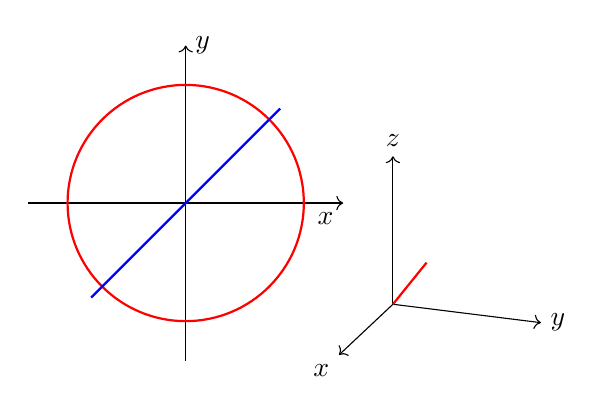
\begin{tikzpicture}
	\begin{scope}[shift={(-4,0)}]
		\draw[->] (-2,0) -- (2,0) node[below left]{$x$};
		\draw[->] (0,-2) -- (0,2) node[right]{$y$};
		\draw[thick, red] (0,0) circle (1.5);
		\draw[thick, blue] (-1.2,-1.2) -- (1.2,1.2);
	\end{scope}
	\tdplotsetmaincoords{70}{110}
	\begin{scope}[tdplot_main_coords, shift={(4,0)}]
		\draw[->] (0,0,0) -- (2,0,0) node[below left]{$x$};
		\draw[->] (0,0,0) -- (0,2,0) node[right]{$y$};
		\draw[->] (0,0,0) -- (0,0,2) node[above]{$z$};
		\draw[thick, red] (0,0,0) -- (1.5,1,1.2);
	\end{scope}
\end{tikzpicture}
\end{lstlisting}

\begin{center}
	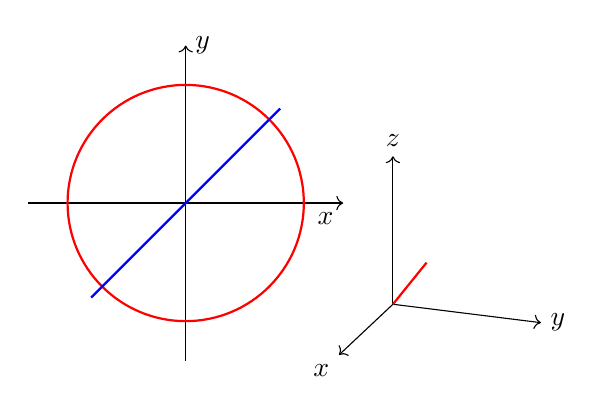
\begin{tikzpicture}
		\begin{scope}[shift={(-4,0)}]
			\draw[->] (-2,0) -- (2,0) node[below left]{$x$};
			\draw[->] (0,-2) -- (0,2) node[right]{$y$};
			\draw[thick, red] (0,0) circle (1.5);
			\draw[thick, blue] (-1.2,-1.2) -- (1.2,1.2);
		\end{scope}
		\tdplotsetmaincoords{70}{110}
		\begin{scope}[tdplot_main_coords, shift={(4,0)}]
			\draw[->] (0,0,0) -- (2,0,0) node[below left]{$x$};
			\draw[->] (0,0,0) -- (0,2,0) node[right]{$y$};
			\draw[->] (0,0,0) -- (0,0,2) node[above]{$z$};
			\draw[thick, red] (0,0,0) -- (1.5,1,1.2);
		\end{scope}
	\end{tikzpicture}
\end{center}

\section{进阶技巧}

\subsection{图文并排（minipage）}
使用 \texttt{minipage} 可以将文档分为左右两部分，一边放文字，一边放图片。这在撰写试卷的时候能派上用场。

\begin{lstlisting}
\noindent
\begin{minipage}[t]{0.6\textwidth} %这里的[t]搭配下面的[t]可以保证图片在minipage的上面，与图片与文字第一行对齐
	这里展示如何在左边写内容，图片展示在右边：\\
	使用minipage.\\
	我们先画了$\triangle ABC$\\
	随后作了$AB$的垂线$CH$\\
	找到了$AB$的中点$M$\\
	将$\triangle ABC$填充了我们定义的LightBlue颜色\\
	又将$A$、$B$、$C$、$H$、$M$分别填充了2pt的红色圆点\\
	$\therefore CH\perp AB$\\
	$\therefore M$是$AB$的中点.
\end{minipage}
\hfill
\begin{minipage}[t]{0.35\textwidth} %这里的[t]可以保证图片在minipage的上面，与图片与文字第一行对齐
	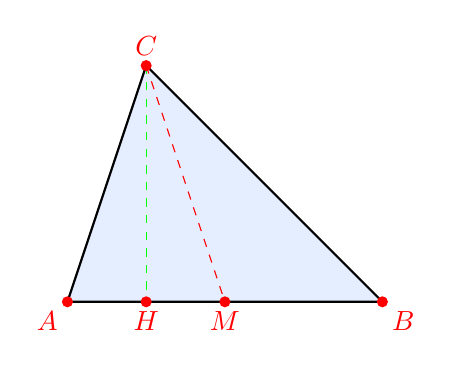
\begin{tikzpicture}[baseline=(current bounding box.north), scale=1] %这里的baseline是调整图片对齐基线的，默认是图片中间，但这明显不是我们想要的，我们想图片顶部对齐文字第一行，而不是图片中间对齐文字第一行，所以改为baseline=(current bounding box.north)，north就是北边（上面），即图片最上面；scale是调整图片整体大小的，但是我们已经规定了minipage的比例了，这里不做调整
		\coordinate (A) at (0,0);
		\coordinate (B) at (4,0);
		\coordinate (C) at (1,3);
		\fill[LightBlue] (A) -- (B) -- (C) -- cycle;
		\draw[thick] (A) -- (B) -- (C) -- cycle;
		\coordinate (M) at ($(A)!0.5!(B)$);
		\draw[dashed, red] (C) -- (M);
		\coordinate (H) at ($(A)!(C)!(B)$);
		\draw[dashed, green] (C) -- (H);
		\foreach \p/\pos in {A/below left, B/below right, C/above, M/below, H/below}
		\fill[red] (\p) circle (2pt) node[\pos] {$\p$};
	\end{tikzpicture}
\end{minipage}
\end{lstlisting}

\noindent
\begin{minipage}[t]{0.6\textwidth}
	这里展示如何在左边写内容，图片展示在右边：\\
	使用minipage.\\
	我们先画了$\triangle ABC$\\
	随后作了$AB$的垂线$CH$\\
	找到了$AB$的中点$M$\\
	将$\triangle ABC$填充了我们定义的LightBlue颜色\\
	又将$A$、$B$、$C$、$H$、$M$分别填充了2pt的红色圆点\\
	$\therefore CH\perp AB$\\
	$\therefore M$是$AB$的中点.
\end{minipage}
\hfill
\begin{minipage}[t]{0.35\textwidth}
	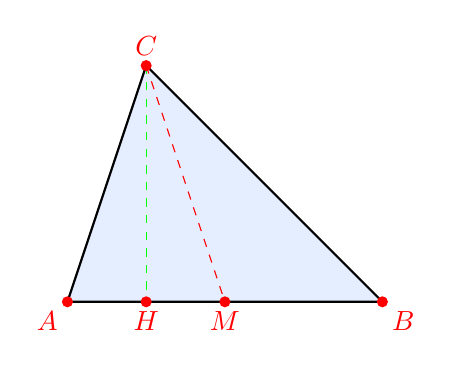
\begin{tikzpicture}[baseline=(current bounding box.north), scale=1]
		\coordinate (A) at (0,0);
		\coordinate (B) at (4,0);
		\coordinate (C) at (1,3);
		\fill[LightBlue] (A) -- (B) -- (C) -- cycle;
		\draw[thick] (A) -- (B) -- (C) -- cycle;
		\coordinate (M) at ($(A)!0.5!(B)$);
		\draw[dashed, red] (C) -- (M);
		\coordinate (H) at ($(A)!(C)!(B)$);
		\draw[dashed, green] (C) -- (H);
		\foreach \p/\pos in {A/below left, B/below right, C/above, M/below, H/below}
		\fill[red] (\p) circle (2pt) node[\pos] {$\p$};
	\end{tikzpicture}
\end{minipage}

\subsection{使用循环绘制多个图形}
利用 \verb|\foreach| 快速绘制多个相似对象。

\begin{lstlisting}
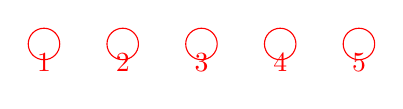
\begin{tikzpicture}
	\foreach \x in {1,...,5}
	\draw[red] (\x,0) circle (0.2) node[below] {$\x$};
\end{tikzpicture}
\end{lstlisting}

\begin{center}
	
\begin{tikzpicture}
		\foreach \x in {1,...,5}
		\fill (\x,0) circle (2pt) node[below] {$\x$};
	\end{tikzpicture}
\end{center}

\subsection{自定义箭头样式}
使用 \texttt{arrows.meta} 库定义箭头。

\begin{lstlisting}
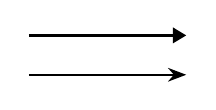
\begin{tikzpicture}
	\draw[->, >=Stealth, thick] (0,0) -- (2,0);
	\draw[->, >=Triangle, thick] (0,0.5) -- (2,0.5);
\end{tikzpicture}
\end{lstlisting}

\begin{center}
	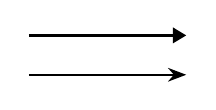
\begin{tikzpicture}
		\draw[->, >=Stealth, thick] (0,0) -- (2,0);
		\draw[->, >=Triangle, thick] (0,0.5) -- (2,0.5);
	\end{tikzpicture}
\end{center}

\subsection{阴影与渐变}
利用 \texttt{shadings} 库添加渐变填充。

\begin{lstlisting}

\begin{tikzpicture}
	\shade[left color=blue, right color=red] (0,0) rectangle (2,1);
\end{tikzpicture}
\end{lstlisting}

\begin{center}
	
\begin{tikzpicture}
		\shade[left color=blue, right color=red] (0,0) rectangle (2,1);
	\end{tikzpicture}
\end{center}

\section{结语}
本教程介绍了使用 \texttt{TikZ} 和 \texttt{tikz-3dplot} 绘制平面与三维图形的基本方法，并涵盖了许多实用技巧。我认为\texttt{pgfplots}比\texttt{TikZ}难学，故不涉及\texttt{pgfplots}的内容，适合从零开始学习。读者可在此基础上进一步探索更多绘图库和样式，如 \texttt{decorations}、\texttt{shadings} 等，以创作更精美的图形。

\newpage
\begin{center}
	{\huge \textbf{附录}}
\end{center}

本教程使用的模板如下，读者可以参考本文档的字体、标题样式、lstlisting设置以及添加的宏包等。

\begin{verbatim}
	\documentclass{article}
	\usepackage{geometry}
	\geometry{
		a4paper,
		left=2.5cm,   
		right=2.5cm,   
		top=2.5cm,      
		bottom=2.5cm,  
		headheight=13.6pt
	}
	
	% 最简单、最稳定的中文方案（自动适配系统，永不报错）
	\usepackage[UTF8, scheme=plain]{ctex}
	
	% 设置英文默认字体为 Times New Roman
	\usepackage{fontspec}
	\setmainfont{Times New Roman}
	
	\usepackage{amsmath}
	\usepackage{amssymb}
	\usepackage{booktabs}
	\usepackage{caption}
	\usepackage{setspace}
	\onehalfspacing
	\setlength{\parskip}{4pt}
	
	\usepackage{array}
	\usepackage{listings}
	\usepackage{graphicx}
	\usepackage{enumitem}
	\usepackage{subcaption}
	\usepackage{multirow}
	\usepackage{mathrsfs}
	\usepackage{bm}
	\usepackage{xcolor}
	\usepackage{colortbl}
	
	\usepackage{tikz}
	\usepackage{tikz-3dplot}
	\usetikzlibrary{
		arrows.meta, 
		calc, 
		patterns, 
		decorations.pathmorphing, 
		backgrounds, 
		positioning, 
		fit, 
		shapes.geometric, 
		intersections, 
		through, 
		angles, 
		quotes,
		plotmarks
	}
	
	%目录超链接
	\usepackage{hyperref}
	\hypersetup{
		colorlinks=true,
		linkcolor=black,
		filecolor=magenta,      
		urlcolor=cyan,
	}
	\usepackage{tocloft}
	\setlength{\cftbeforesecskip}{2ex}
	\setlength{\cftbeforesubsecskip}{1ex}
	\setlength{\cftbeforesubsubsecskip}{1ex}
	
	% 定义代码颜色
	\definecolor{codegreen}{rgb}{0,0.6,0}
	\definecolor{NavyBlue}{RGB}{0,0,128}
	\definecolor{PineGreen}{RGB}{1,121,111}
	
	% 配置 listings 环境
	\lstset{
		language=TeX,
		tabsize=4,
		captionpos=b,
		numbers=left,
		numbersep=1em,
		sensitive=true,
		showtabs=false,
		frame=shadowbox,
		breaklines=true,
		keepspaces=true,
		showspaces=false,
		showstringspaces=false,
		breakatwhitespace=false,
		basicstyle=\ttfamily\normalsize,
		keywordstyle=\color{NavyBlue},
		commentstyle=\color{codegreen},
		numberstyle=\color{black},
		stringstyle=\color{PineGreen!90!black},
		rulesepcolor=\color{red!20!green!20!blue!20},
		escapeinside={/@}{@/},
	}
	
	\definecolor{LightGreen}{rgb}{0.9, 0.95, 0.9}
	\definecolor{LightBlue}{RGB}{229, 238, 255}
	\definecolor{LightPink}{RGB}{255, 229, 237}
	
	\captionsetup[table]{
		justification=centering,
		labelsep=quad,
		font={bf}
	}
	\captionsetup[figure]{
		justification=centering,
		labelsep=quad,
		font={bf}
	}
	\captionsetup[subfigure]{
		font={bf}
	}
	
	\begin{document}
		...
	\end{document}
\end{verbatim}
\end{document}